\newcommand\imagenetwidth{0.45}
\begin{figure*}[ht]
\vspace{-8pt}
\centering
\begingroup
\setlength{\tabcolsep}{2pt}
\begin{tabular}{cccc}
\rotatebox[origin=c]{90}{\small{ImageNette}}    &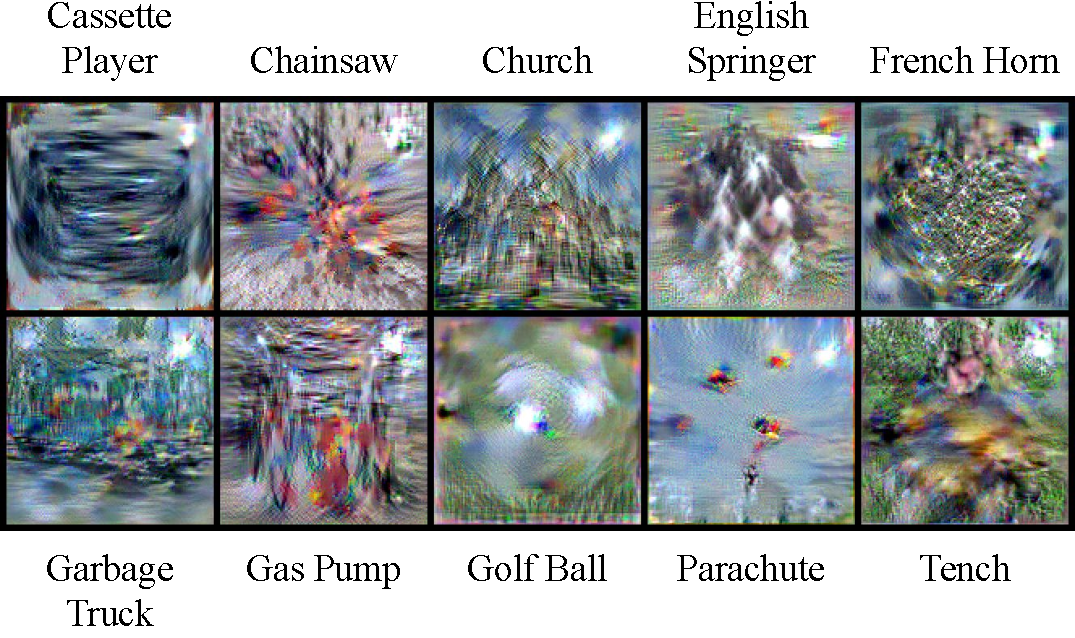
\includegraphics[align=c,width=\imagenetwidth\linewidth]{figures/ImageNette.pdf}
    &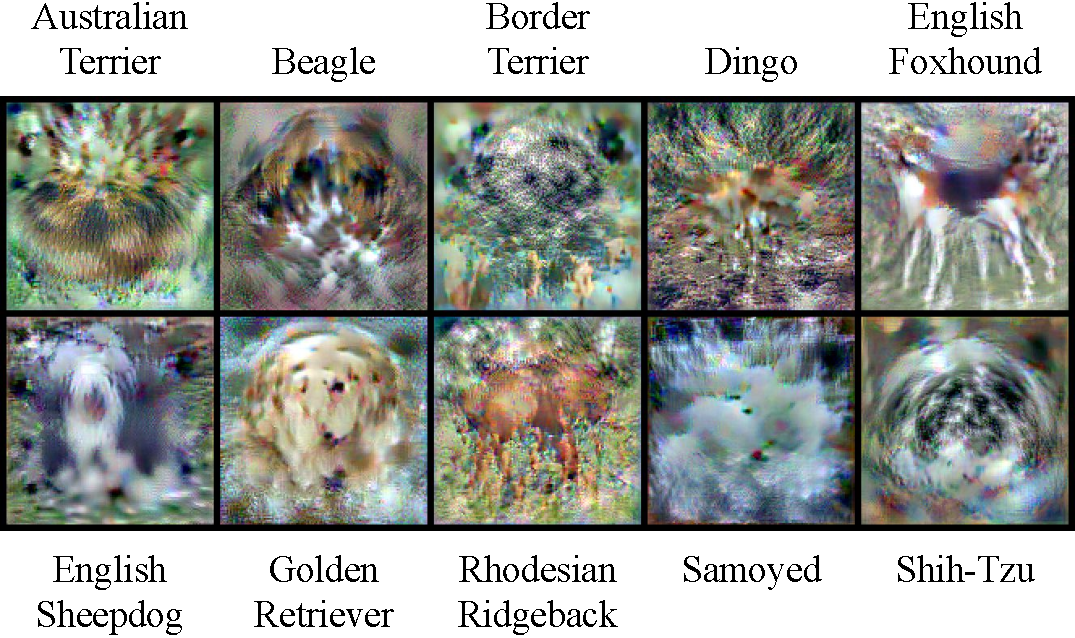
\includegraphics[align=c,width=\imagenetwidth\linewidth]{figures/ImageWoof.pdf} & \rotatebox[origin=c]{270}{\small{ImageWoof}} \\[-0.8ex]
\rotatebox[origin=c]{90}{\small{ImageSquawk}}    &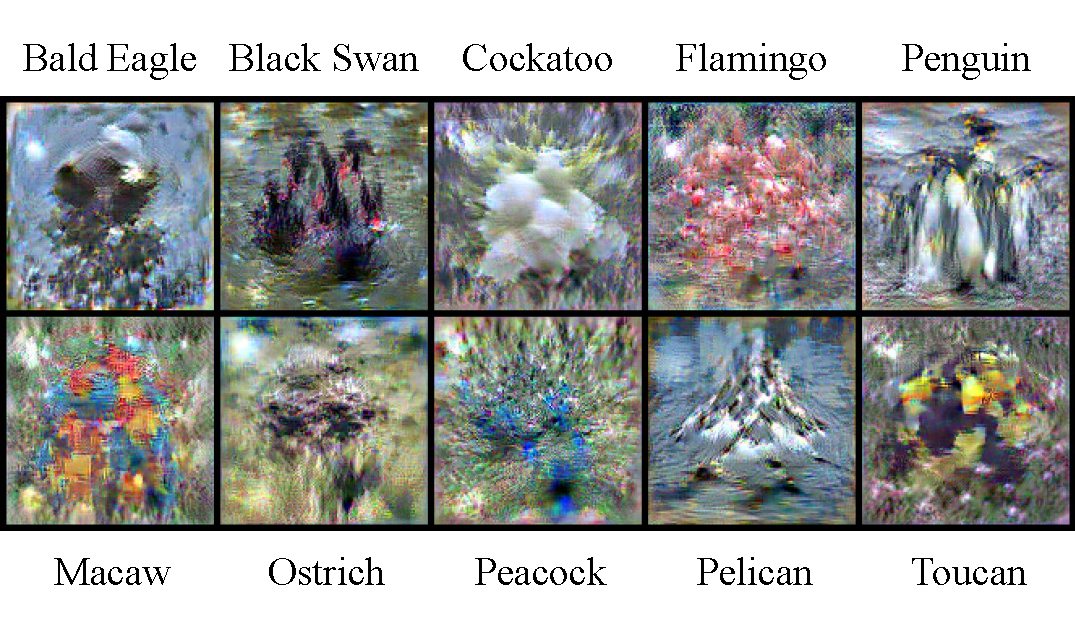
\includegraphics[align=c,width=\imagenetwidth\linewidth]{figures/ImageSquawk.pdf}
    &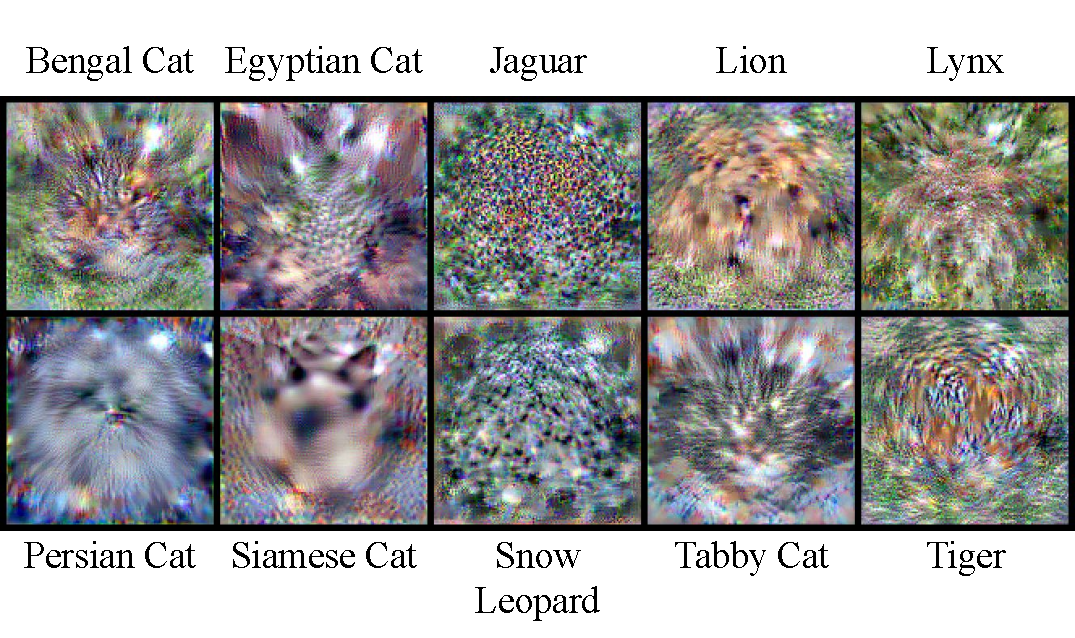
\includegraphics[align=c,width=\imagenetwidth\linewidth]{figures/ImageMeow.pdf} & \rotatebox[origin=c]{270}{\small{ImageMeow}} \\[-0.8ex]
\rotatebox[origin=c]{90}{\small{ImageFruit}}    &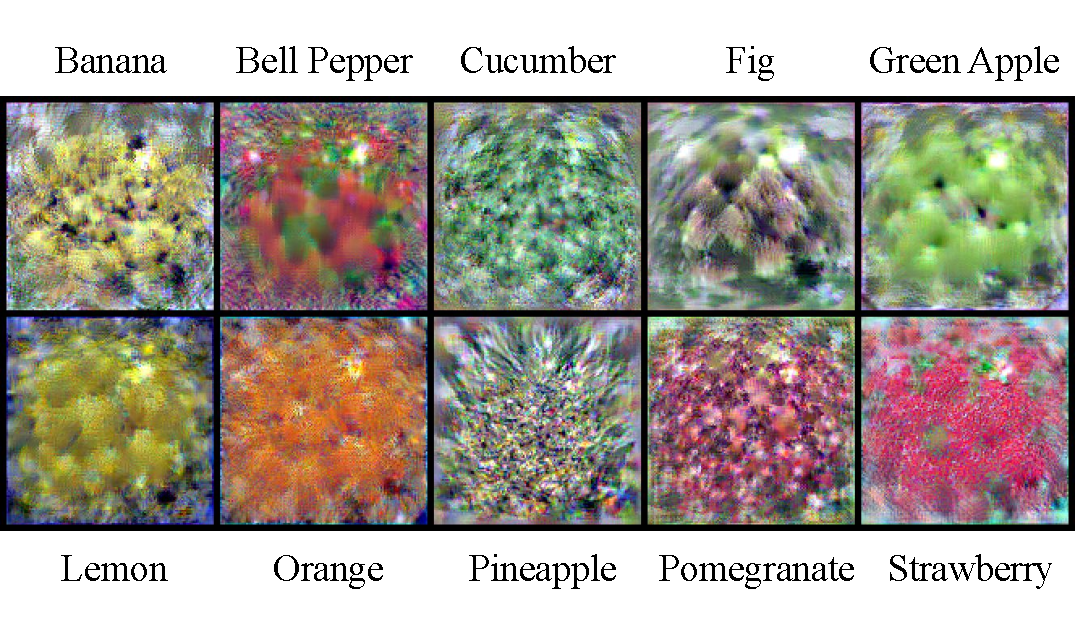
\includegraphics[align=c,width=\imagenetwidth\linewidth]{figures/ImageFruit.pdf}
    &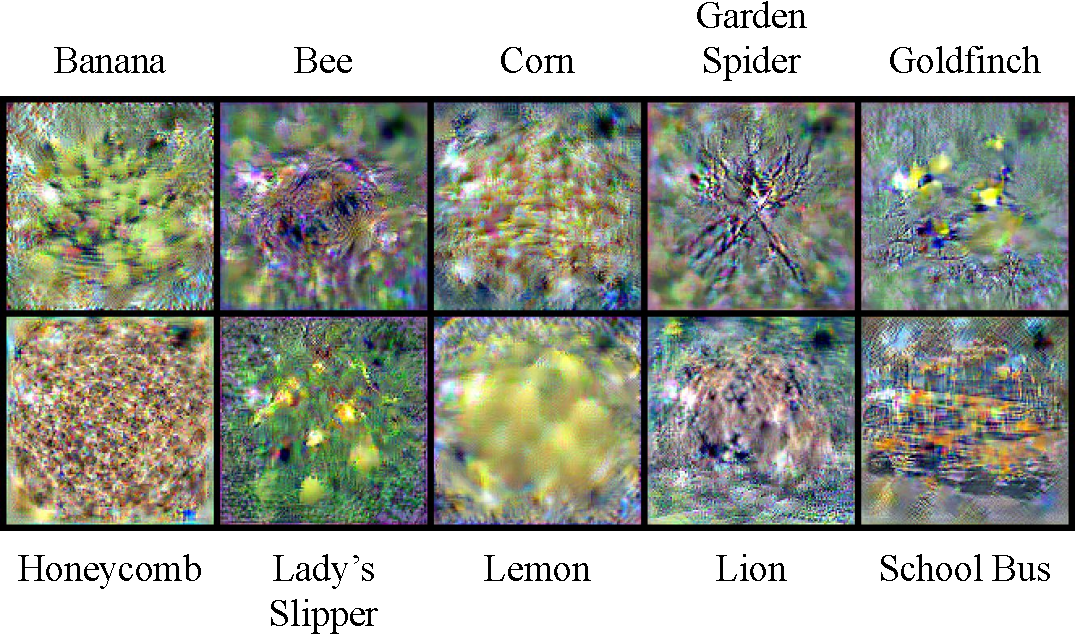
\includegraphics[align=c,width=\imagenetwidth\linewidth]{figures/ImageYellow.pdf} & \rotatebox[origin=c]{270}{\small{ImageYellow}}
\end{tabular}
\endgroup
\vspace{-0.3cm}
    \captionof{figure}{Our method is the first capable of distilling higher-resolution (128$\times$128) images, allowing us to explore the ImageNet \cite{deng2009imagenet} dataset.}
    \lblfig{imagenet}
    \vspace{-6pt}
\end{figure*}

